\section{Related Work}
\label{sec:related}
OppNets, which face two challenges,
i.e., energy efficiency and network management cost,
are expected to accommodate participants
with low-delay and cost-effective services.
Therefore, many research works targeted to address these issues.

\subsection{Message Relaying in OppNets}
The primary goal of message forwarding in OppNets
is to exploit the nodes' contact, context,
and social information to improve
the message delivery performance
in terms of different metrics (e.g.,
delivery ratio, delay, overhead,
energy consumption and privacy).
Geo-casting routing protocols, like 
LoSeRo~\cite{DBLP:journals/tmc/CostantinoMMS20},
exploited knowledge of the most frequently visited
to route message in OppNets
and achieved a significant high delivery rate.
Then onion-based anonymous routing
approach~\cite{DBLP:conf/icdcs/SakaiSKWA16}
and ePRIVO~\cite{DBLP:journals/tvt/MagaiaBPC18} were 
proposed to keep users' information private.
To achieve the tradeoff between the delivery ratio
and forwarding cost,
game theory was introduced to
optimize the network configuration in MANETs
for more efficient energy-aware routing
in~\cite{DBLP:journals/monet/MaoZ15}.
%For MOSNs, which exhibits 
Based on a Nested Core-Periphery Hierarchy (NCPH),
\cite{DBLP:journals/tvt/Zheng017} presented
an up-and-down routing protocol,
which can achieve the proper balance
among the data delivery delay, ratio, and cost.
\cite{DBLP:journals/adhoc/RosasGH20} proposed
a context-aware self-adaptive routing protocol
that is able to adapt to different scenarios.

The majority of aforementioned protocols
assume that mobile nodes are willing 
to participate in data delivery.
Nevertheless,
rational nodes in OppNets have strategic interactions
and may exhibit selfish behaviors.
In order to mitigate the performance degradation
caused by the selfishness,
much effort has been made to explore
appropriate incentive mechanisms
to encourage selfish nodes to
participate in data relaying.
For example, the tit-for-tat (TFT)-based scheme,
which forces nodes to exchange the same number
of messages during an opportunistic contact,
was introduced to ensure that 
mobile nodes provide better forwarding services 
for cooperative nodes,
and protect the network against the harm of selfish behaviors
in~\cite{DBLP:journals/tmc/MastronardePXLS16,
DBLP:journals/twc/HsuD17}.
Trust and reputation-based
schemes were adopted to build direct trust relationships
or indirect trust recommendations 
among mobile
nodes~\cite{DBLP:journals/tvt/ChenLWW16,DBLP:conf/mdm/JethawaM18}.
Eventually, better services were provided
for nodes with high reputation
or strong trust relationships.
Credit-based schemes, such as SEIR~\cite{DBLP:conf/ciss/ChhabraVS17},
Multicent~\cite{DBLP:journals/tpds/ChenSY15},
were designed to encourage the node participation
in data relaying 
by rewarding the cooperative nodes
and punishing the selfish nodes.
%via various virtual credits.
%by employing various forms
%of the virtual credit to

\subsection{Abnormal Behavior Detections in OppNets}
\begin{figure}
  \centering
  {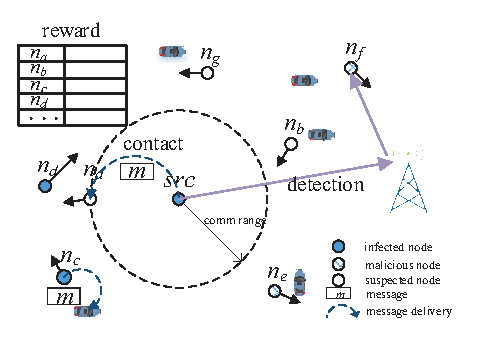
\includegraphics[width=0.47\textwidth]{fig/sketch.eps}}
     \caption{Reward and detection of the selfish nodes in OppNets.}
     \label{fig:sketch}
\end{figure}
Due to the openness of
the wireless communication and the limitations of the
`store-carry-forward' paradigm,
the performance of data delivery in OppNets may be reduced
by abnormal behaviors.
For example,
the selfish behaviors will seriously degrade
the efficiency of data offloading
and the malicious behaviors
will disrupt the normal communications 
between the nodes and the network
throughput deeply~\cite{DBLP:journals/comsur/JedariXN18}.
It is critical to
identify the abnormal node behaviors from network accurately 
and promote the participation of nodes
in the data relaying and the resource sharing.

Observing the importance of selfish behavior detection
schemes for the OppNets,
%the research attentions were attracted in
%a lot of efforts were
a lot of works were
put into its design~\cite{DBLP:journals/fgcs/JedariXCDTA19, Zhou2015Incentive, Chen2014Dynamic, DBLP:journals/tdsc/ChoC18, Wang2016A}.
In~\cite{DBLP:journals/fgcs/JedariXCDTA19},
a general altruism model,
called SoWatch,
was utilized to
distinguish individually selfish behavior 
and socially selfish behavior.
It also showed that the individual 
and social preferences of selfish nodes
may mitigate the cooperation in data relaying.
An incentive-driven and freshness-aware 
pub/sub content dissemination scheme
was proposed in~\cite{Zhou2015Incentive},
with the objective of 
maximizing the utility of the content inventory 
stored in node's buffer.
\cite{Chen2014Dynamic} proposed a dynamic trust management protocol,
in which `healthiness' and
`unselfishness' are considered as two social trust metrics.
A more comprehensive set of performance metrics to characterize QoS (Quality of Service)
in the OppNets
was investigated in~\cite{DBLP:journals/tdsc/ChoC18}.
To guaranty the security requirements of the OppNets,
a credit-based
rewarding scheme was proposed in~\cite{Wang2016A}.

On the other hand,
the protection and defense mechanisms for malicious behaviors have
been demanded by the OppNets.
To deal with the blackhole and greyhole attacks
in DTNs,
\cite{Pham2016Detecting} proposed 
a statistical-based detection scheme and
demonstrated its high accuracy.
A secured routing algorithm for the DTNs
was proposed in~\cite{Saha2018Design},
where the information list of malicious nodes 
was delivered by the trusted nodes.
The types and effectiveness of Sybil attacks in OppNets
was introduced by~\cite{Sacha2016Stalk},
with the consideration of various resource and
attack boosting graph faking attempts.
The problem of confidence crisis caused by malicious nodes
was proposed in~\cite{Yao2016Secure},
and a dynamic trust management model
was presented there to solve the problem.
In~\cite{Chen2016Trust},
an adaptive trust management
protocol for social IoTs (Internet of Things) systems was proposed
to choose the trust parameter settings and change node's social conditions.
%Optimization schemes of OppNets can be classified into
%several types, the most typical one tries to formulate
%the transmitting process in terms of a trade-off between
%the network management cost and the transmission performance.
%For example, on optimal neighbor discovery,
%PWEND~\cite{DBLP:journals/adhoc/ChenQLLWYL20} and
%Pharos~\cite{DBLP:conf/secon/Zhu00L19} adopted time model
%for neighbor discovery and investigated the most energy efficient way
%and the least discovery latency, respectively.
%Then for a given energy budget,
%how to optimizing the number of discovered peers was researched
%in~\cite{DBLP:journals/tmc/LoretiB20},
%what is the best achievable discovery latency was addressed
%by~\cite{DBLP:conf/sigcomm/KindtC19}.
%
%As for optimal data forwarding,
%\cite{DBLP:journals/tvt/ZhouLZXF17} proposed an
%efficient time-aware data forwarding strategy(TCCB) for OMNs,
% based on temporal social contact patterns.
% The model performed a close delivery ratio to
% Epidemic but with significantly reduced delivery cost.
%\cite{DBLP:journals/tvt/LiuWXWLY17} introduced
%a centralized heuristic algorithm
%which aimed to discover a tree for multicasting,
%with resource constrained (i.e. the delay-constrained least-const) in MONs.
%Both centralized and decentralized single-copy message forwarding algorithms
%were proposed in~\cite{DBLP:journals/tsipn/ShaghaghianC15},
%which aimed to minimize the expected latencies
%from any node in the Opportunistic DTNs.
%However, aforementioned works just consider one part of
%the message transmission in OppNets,
%\cite{DBLP:journals/tcss/WuDH18} mathematically characterized
%message transmission of the selfish
%and altruistic cases as an optimal control problem,
%whose controlling parameters were chosen according
%to the forwarding rate and beaconing rate, respectively.
%Then the Pontryagin's Maximum Principle was exploited
%to search the problem solution in multiple destinations scenario
%and the optimal control policies were proved to satisfy the threshold form.
%%Wu et al. considered the optimal forwarding and beaconing control problem at the same time in DTN and gave solution based on Pontryagin's Maximum Principle in ~\cite{DBLP:journals/tcss/WuDH18}, where multiple destinations exist.
%
%Minimize the contact duration by optimizing
%mobile data offloading in OMNs is the objective
%of~\cite{DBLP:journals/tits/LiJWZ014,DBLP:conf/icc/WangW18}.
%A mathematical framework to study the problem of
%coding-based mobile data offloading
%was established in~\cite{DBLP:journals/tits/LiJWZ014},
%the authors formulated the problem as a users' interest
%satisfaction maximization problem
%with multiple linear constraints of
%limited storage and efficient scheme
%was proposed to solve it.
%An optimal traffic offloading scheme through
%data partition, which generated forwarding paths
%with possible heterogeneous data chunks,
%was presented in~\cite{DBLP:conf/icc/WangW18}.

%Few these existing works focus on
%optimal control policy, while we introduce it
%for selfish node detection,
%where the scenario is different
%from~\cite{DBLP:journals/tcss/WuDH18} in this paper.
Few existing works focus on
the optimal control policy to balance
the cost of selfish node detection
and the reward to encourage the participation of nodes.
Therefore, we utilize ODEs to model the message dissemination
caused by contacts and detections,
and propose a optimal selfish node detection method
based on the Pontryagin's maximum principle.
